\section{The C-{}- language}
In this section we present the implementation of a small imperative language called C-{}-. Note that, although the name might suggest this, we do not claim any resemblance with the C programming language, as it lacks several features such as pointer arithmetic, arrays, and functions.

C-{}- allows the use of four built-in values: integer, strings, booleans, and floating-point numbers in double precision. The memory is represented using a dictionary that pairs variable names with their value. In what follows we omit the details of the lookup of entries in the dictionary for brevity. Suffice to say that the meta-program makes use of the \texttt{ImmutableDictionary} data structure available in .NET. Also note that C-{}- defines scopes for variables, so that if a variable is declared inside the scope of a code block in a control structure, that is usable only within the scope itself.

The core of the meta-program is made of the evaluation of both expressions and statements. We proceed below to present the details of both kinds of evaluation.

\subsection{Expression Semantics}
As explained above C-{}- supports boolean, string, integer, and floating-point values. These are represented through the following meta-data structures in the meta-program.

\begin{lstlisting}
Data "$i" -> <<int>> : Value Priority 300
Data "$d" -> <<double>> : Value Priority 300
Data "$s" -> <<string>> : Value Priority 300
Data "$b" -> <<bool>> : Value Priority 300
\end{lstlisting}

\noindent
Note that we are using the .NET data types to represent the actual values stored in the meta-data structures. We also define the following type equivalence, since values are atomic cases of expressions and can be used as such:

\begin{lstlisting}
Value is Expr
\end{lstlisting}

\noindent
Expressions can also contain variables, thus we need a meta-data structure to represent them as well.

\begin{lstlisting}
Data "$" -> <<string>> : Id Priority 300
\end{lstlisting}

\noindent
Variables can be used as atomic expressions as well, so we need an additional type equivalence

\begin{lstlisting}
Id is Expr
\end{lstlisting}

\noindent
We now define a data structure to represent the state of the program. The state is simply a map where the key is a variable name and the stored element a valid value in C-{}-. In the declaration we will define the meta-type \texttt{SymbolTable}, and from now on we will refer use the term ``symbol table'' as a synonym of ``state''.

\begin{lstlisting}
Data "$m" << ImmutableDictionary<Id, Value> >> : SymbolTable 
\end{lstlisting}

\noindent
Since we want to allow variable scoping, the state of the program is not represented by a single map, but by a list of maps. Each time the program enters a different scope context, an empty map is added to this list, and removed when the program exits the scope. This process will be further explained below. We define a meta-data structure to represent this list of states (note that the operator for the construction of the list is infix).

\begin{lstlisting}
Data SymbolTable -> "::" -> TableList : TableList
\end{lstlisting}

\noindent
We can finally proceed to define a meta-data structure to represent the operations for expressions. First we define the arithmetic operators in the language:

\begin{lstlisting}
Data Expr -> "+" -> Expr : Expr
Data Expr -> "-" -> Expr : Expr
Data Expr -> "*" -> Expr : Expr
Data Expr -> "/" -> Expr : Expr
\end{lstlisting}

\noindent
then we can define operators for boolean expressions:
\begin{lstlisting}
Data Expr -> "&&" -> Expr : Expr
Data Expr -> "||" -> Expr : Expr
Data "!" -> Expr : Expr
\end{lstlisting}

\noindent
and finally comparison operators:
\begin{lstlisting}
Data Expr -> "equals" -> Expr : Expr
Data Expr -> "neq" -> Expr: Expr
Data Expr -> "ls" -> Expr : Expr
Data Expr -> "leq" -> Expr : Expr
Data Expr -> "grt" -> Expr : Expr
Data Expr -> "geq" -> Expr : Expr
\end{lstlisting}

We now have to define the function that evaluates an expression through rules in the program. This function takes as input the list of symbol tables (needed to read possible variables), an expression, and returns the value after computing the expression.

\begin{lstlisting}
Func "evalExpr" -> TableList -> Expr : Value
\end{lstlisting}

\noindent
Now we have to proceed to define the rules to compute the actual evaluation of an expression. Clearly the base cases of the evaluation are the atomic values, where we immediately return the value itself.

\begin{lstlisting}
-----------------------------
evalExpr tables ($i v) -> ($i v)

-----------------------------
evalExpr tables ($d v) -> ($d v)

-----------------------------
evalExpr tables ($s v) -> ($s v)

-----------------------------
evalExpr tables ($b v) -> ($b v)
\end{lstlisting}

Evaluating variables is more complex: we have to look at the table currently in the head of the list of tables (which is the one relative to the current scope). If we do not find the required variable we have to recursively look it up in the tail of the list, since we could have an arbitrary amount of nested scopes. When the variable is found we return its value. This behaviour is implemented by the following code:

\begin{lstlisting}
symbols contains ($name) -> Yes
symbols lookup ($name) -> val
-------------------------------------------
evalExpr (symbols :: tables) ($name) -> val

symbols contains ($name) -> No
evalExpr tables ($name) -> val
-------------------------------------------
evalExpr (symbols :: tables) ($name) -> val

\end{lstlisting}

We proceed now to define the evaluation of arithmetic operators. We show only the example of the sum for brevity, the other rules differ only in the operator. Evaluating the arithmetic expression requires to recursively call \texttt{evalExpr} on the right and left argument. These recursive calls will eventually return two values that are the result of the two evaluations. After we obtain these values, we can compute their sum and return it as result.

\begin{lstlisting}
evalExpr tables expr1 -> ($i val1)
evalExpr tables expr2 -> ($i val2)
<<val1 + val2>> -> v
---------------------------------------
evalExpr tables expr1 + expr2 -> ($i v)
\end{lstlisting}

\noindent
Note that we have used .NET external code in the third premise to compute the result of the arithmetic operation. Evaluating arithmetic operations involving floating-point expressions can be done in an analogous way, except in the premises we expect to have the meta-data structure for floating-point values as result of \texttt{evalExpr}:

\begin{lstlisting}
evalExpr tables expr1 -> ($d val1)
evalExpr tables expr2 -> ($d val2)
<<val1 + val2>> -> v
---------------------------------------
evalExpr tables expr1 + expr2 -> ($d v)
\end{lstlisting}

\noindent
The same can be said for the string concatenation.
The evaluation of boolean expression is analogous: we show again only the evaluation for AND as the other rules are analogous:

\begin{lstlisting}
evalExpr tables expr1 -> ($b val1)
evalExpr tables expr2 -> ($b val2)
<<val1 && val2>> -> b
----------------------------------------------------------------------
evalExpr tables expr1 && expr2 -> b
\end{lstlisting}

\noindent
Again we rely on external code to compute the actual boolean value.
As for the comparison operators, we can use a clause in the premise to avoid using external code in the following way:

\begin{lstlisting}
evalEpxr tables expr1 -> val1
evalExpr tables expr2 -> val2
val1 == val2
------------------------------------------------
evalExpr tables (expr1 equals expr2) -> $b true

evalEpxr tables expr1 -> val1
evalExpr tables expr2 -> val2
val1 != val2
------------------------------------------------
evalExpr tables (expr1 equals expr2) -> $b false
\end{lstlisting}

\noindent
The first rule checks that the values computed by evaluating the left and right argument of the equality comparison are the same. If this happens then the rule returns a meta-data structure containing the boolean representation of \texttt{true}. Otherwise the first rule fails and the second one is executed. This one will return a boolean representation of \texttt{false} when the values are different.

For inequality operators we must rely on external code for the computation is Metacasanova only allows equality comparisons in clauses:

\begin{lstlisting}
evalExpr tables expr1 -> ($i val1)
evalExpr tables expr2 -> ($i val2)
<< val1 < val2 >> -> boolResult
---------------------------------------------------------
evalExpr tables (expr1 ls expr2) -> ($b boolResult)
\end{lstlisting}

\noindent
The evaluation of the other comparison operators is implemented through analogous rules, which differ only in the operators.

\subsection{Statement Semantics}

Statement evaluation requires the definition of a different function, \texttt{eval}, that processes each statement and returns the result of the statement evaluation and the updated state. Note that, even if the evaluation of statements does not always change the state, in general we have to assume that this will happen.

The function \texttt{eval} takes as input a statement to process and the current state (list of symbol tables), and returns the updated list of symbol tables

\begin{lstlisting}
Func "eval" -> TableList -> Stmt : TableList
\end{lstlisting}

We now proceed to define the meta-data structures necessary to represent the statements of the language: C-{}- supports (\textit{i}) variable declarations, (\textit{ii}) variable assignment, (\textit{iii}) if-then-else, (\textit{iv}) while loops, and (\textit{v}) for loops.

Variable declarations follow the same structure of standard C, that is a type name followed by an identifier. Thus, the corresponding meta-data structure can be defined as:

\begin{lstlisting}
"variable" -> Type -> Id : Stmt
\end{lstlisting}

\noindent
Analogously, variable assignment follows the C convention and uses the \texttt{=} symbol.

\begin{lstlisting}
Id -> "=" -> Expr : Stmt
\end{lstlisting}

The control structure if-then-else does not follow the standard C representation, rather we use the keywords \texttt{then} and \texttt{else} to delimit its code blocks. Note that nothing would prevent to implement the conventional C syntax, but we prefer this ``lightweight'' representation. The keywords \texttt{then} and \texttt{else} are meta-data structures that take no arguments and do not have any functional utility other than syntactical mark-ups.

\begin{lstlisting}
Data "then" : Then
Data "else" : Else
Data "if" -> Expr -> Then -> Stmt -> Else -> Stmt : Stmt
\end{lstlisting}

Analogously we can define the meta-data structure for \texttt{While} and \texttt{For}

\begin{lstlisting}
Data "do" : Do
Data "while" -> Expr -> Do -> Stmt : Stmt
Data "for" -> Expr -> Expr -> Epxr -> Do -> Stmt : Stmt
\end{lstlisting}

\noindent
Up to this point we are able to define single statements in the language, but we need a way to concatenate a sequence of statements to form code blocks, in the fashion of C. This is done by introducing an additional meta-data structure, which is the ";" symbol. For convenience, we also introduce a \texttt{nop} statement, which does not do anything, but it will be useful to express the semantics of statements evaluation.

\begin{lstlisting}
Data Stmt -> ";" -> StmtList : StmtList
Data "nop" -> :Stmt

StmtList is Stmt

\end{lstlisting}

We now proceed to define the semantics of statement evaluation. 

\subsubsection{Variable Declarations and Assignments}
Evaluating a variable declaration simply adds the variable to the symbol table of the current scope. Note that we allow variable shadowing, so it is possible to redefine the same symbol in different scopes.

\begin{lstlisting}
symbols defineVariable id -> symbols'
-------------------------------------
eval (symbols nextTable tables) (variable t id) -> symbols' nextTable tables
\end{lstlisting}

\noindent
This rule is executed whenever the processed statement matches the structure of a variable declaration statement. The premise adds the symbol to the symbol table of the current scope (we omit the details for brevity), and returns an updated symbol table. The list of symbol 
tables is rebuilt to include the updated table and returned as result.

Variable assignment is more complex, since the variable we are trying to use might not be in the symbol table of the current scope. We must then define two lookups functions, that behave differently depending on whether the variable is in the symbol table in the head of the symbol table list or not. We declare the function \texttt{updateTable} that performs this lookup and updates the table list accordingly. 

\begin{lstlisting}
Func "updateTables" -> TableList -> TableList -> Id -> Expr : EvaluationResult
\end{lstlisting}

\noindent
In the case that the variable is in the symbol table in the head of the list of tables we have the following rule:

\begin{lstlisting}
symbols contains id -> Yes
evalExpr vars expr -> val
symbols add id val -> symbols'
-------------------------------
updateTables vars (symbols nextTable tables) id expr -> symbols' nextTable tables
\end{lstlisting}

\noindent
The first premise checks if the symbol is contained in the table in the head of the list. If the answer is \texttt{Yes} (a meta-data structure returned by the function \texttt{contains}, not described here again for brevity), then the second premise proceeds to evaluate the expression in the right hand-side of the assignment. The third premise adds the value obtained as result of the second premise to the current symbol table and returns the modified table. The new table is than placed in the head of the table list and the whole list is returned. Note that, at this point, all the tables in the list remain unchanged except the one that was in the head. Note that \texttt{updateTables} carries two copies of the list of tables. One of them is passed to \texttt{eval} because the right-hand side of the assignment might contain other variables. The process of looking up the left hand-side variable pops symbol tables from the head of list (see next rule) but the original list of tables is necessary when assigning the values of variables located in inner scopes. For instance, consider the following program in C-{}-:

\begin{lstlisting}[caption = C-{}- sample program, label = code:ch_mcnv_languages_c--_sample_program]
int x;
...
if (x > 0) then
	int y;
	y = 4
	x = y;
else
  x = x - 1;	
\end{lstlisting}

\noindent
assume that before the if-then-else $x > 0$. The program will enter the \texttt{then} block and declare \texttt{y}. In the current state we have to symbol tables, one for the scope of the \texttt{if-then-else} and one for the outer scope. When assigning \texttt{y} to \texttt{x} the symbol table tries to look up \texttt{x} in the table of the current scope and fails. This will pop the head of the list of tables (which is the table of \texttt{if-then-else}) and recursively look in the tail. During the second attempt \texttt{x} is retrieved but now we do not have the symbol table where \texttt{y} is defined anymore to evaluate the right hand-side. We thus need the original list of tables to be able to retrieve \texttt{y}. In general, if we call \texttt{$d_l$} the depth of scoping of the left hand-side and $d_r$ the depth of scoping of the right hand-side, the process pops the table of the right hand-side whenever $d_l > d_r$ and this is when we need the original list of tables to retrieve the value of the right hand-side.

If the variable is not contained in the head of the list, i.e. it has not been declared in the current scope, we have the following rule:

\begin{lstlisting}
symbols contains id -> No
updateTables vars tables id expr -> tables'
----------------------------------------------
updateTables vars (symbols nextTable tables) id expr -> symbols nextTable tables'
\end{lstlisting}

The first premise tries to lookup the variable in the symbol table of the current scope and does not find it. Thus we recursively call \texttt{updateTables} with the tail of the list. The recursive call will eventually find the variable in one of the symbol tables associated with outer scopes. This process will produce an updated list of tables that is returned as a new tail for the current list.

At this point, the rule for the evaluation of the variable assignment simply class the \texttt{updateTables} function in its premise:

\begin{lstlisting}
updateTables tables tables id expr -> res
----------------------------------------
eval tables (id = expr) -> res
\end{lstlisting}

\subsubsection{Conditionals}

Evaluating \texttt{if-then-else} requires two rules, depending on the result of the evaluation of its condition. The following rule implements the semantics when the condition is false:

\begin{lstlisting}
evalExpr tables condition -> $b true
emptyDictionary -> table
eval (table nextTable tables) thenBlock -> table' nextTable tables''
-------------------------------------------------------------------
eval tables (if condition then thenBlock else elseBlock) -> tables''
\end{lstlisting}

The first premise evaluates the condition of the control structures and succeeds if the result is a meta-data structure containing the boolean value \texttt{true}. The second premise uses an utility function to initialize an empty symbol table. This is required to define a new table for the scope of the conditional. The third premise evaluates the statements contained in the then block after pushing the symbol table for the current scope in the list of symbol tables. This process will eventually produce a new list of symbol tables. The result returns only the tail of this list, since when we exit the scope of the conditional we must pop its symbol tables.

For instance, consider again the program in Listing \ref{code:ch_mcnv_languages_c--_sample_program} and again assume that $x > 0$. After executing the then block, the state of the program is made of the symbol tables shown in Table \ref{tab:ch_mcnv_languages_tables_ifthenelse}

\begin{table}
	\centering
	\begin{tabular}{|l|l|}
		\hline
		\textbf{Variable} & \textbf{Value} \\
		\hline
		x & undefined\\
		\hline
	\end{tabular}\\
	\vspace{0.2cm}
	\begin{tabular}{|l|l|}
		\hline
		\textbf{Variable} & \textbf{Value} \\
		\hline
		y & 4\\
		\hline
	\end{tabular}
	\begin{tabular}{|l|l|}
		\hline
		\textbf{Variable} & \textbf{Value} \\
		\hline
		x & 4\\
		\hline
	\end{tabular}
	\caption{Symbol table at the beginning and after the execution of the program in Listing \ref{code:ch_mcnv_languages_c--_sample_program} with $x > 0$}
	\label{tab:ch_mcnv_languages_tables_ifthenelse}
\end{table}

\noindent
After exiting the then block, variable \texttt{y} exits the scope, thus we have to pop the symbol table for the current scope. However, the symbol table of the outer scope has been changed because \texttt{x} got the value of \texttt{y}. Thus the evaluation returns the list containing this updated table. In general, the process should consider that an arbitrary amount of symbol tables for each outer scope have been changed, thus we return this updated list.

The rule that evaluates conditionals when the condition is false is analogous, except this time we evaluate the else block:

\begin{lstlisting}
evalExpr tables condition -> $b false
emptyDictionary -> table
eval (table nextTable tables) elseBlock -> table' nextTable tables''
--------------------------------------------------------------------
eval tables (if condition then thenBlock else elseBlock) -> tables''
\end{lstlisting}

\subsubsection{While Loops}
Evaluating the while loops require to check its condition first. When the condition is false we simply skip the loop without changing the state. The rule to implement this behaviour is thus straightforward:

\begin{lstlisting}
evalExpr tables condition -> $b false
--------------------------------------------
eval tables (while condition expr) -> tables
\end{lstlisting}

\noindent
The semantics when the condition is true is more complex:

\begin{lstlisting}
evalExpr tables condition -> $b true
emptyDictionary -> table
eval (table nextTable tables) block -> table' nextTable tables''
eval tables'' (while condition do block) -> res
---------------------------------------------------
eval tables (while condition do block) -> res
\end{lstlisting}

\noindent
The first premise succeeds when the evaluation of the condition returns a true boolean value in C-{}-. Analogously to what we did for conditionals, we initialize an empty symbol table for the current scope and we push it into the list of symbol tables. We then evaluate the body of the loop. This process will, in general, produce an updated list of symbol tables. Again we pop the symbol table for the current scope because we are exiting the loop. We then evaluate again the whole loop to test its condition again.

\subsubsection{For Loops}
For loops follow the C convention and are made of four parts: (\textit{i}) an initialization, (\textit{ii}) a condition (\textit{ii}), (\textit{iii}) a step, and (\textit{iv}) a block of code. The initialization is evaluated once before entering the loop, the condition is tested before each iteration of the loop, and the step is evaluated at the end of each iteration. In order to implement this behaviour we make use of an additional support function called \texttt{loopFor}:

\begin{lstlisting}
Func "loopFor" -> TableList -> Expr -> Stmt -> Stmt : TableList
\end{lstlisting}

\noindent
The evaluation of the \texttt{for-loop} evaluates the initialization in its premise. It then calls \texttt{loopFor} after the initialization has been evaluated. Again the initialization might define additional variables that enter the scope of the loop, so the updated table of the current scope is pushed into the list of symbol tables. Note that possible variables defined in the initialization part of the loop might be used after the loop itself, according to the semantics of C, so we have to insert them into the symbol table of the current scope and not the one of the loop itself.

\begin{lstlisting}
eval tables init => tables'
loopFor tables' condition step block => res
-------------------------------------------------------
eval tables (for init condition step do block) => res
\end{lstlisting}

The rules for \texttt{loopFor} are two, since we must consider the case when the condition is false and the one where it is true. When the condition is false the loop is completely skipped, thus we simply return the current state without any changes, in the same fashion of the \texttt{while-loop}:

\begin{lstlisting}
evalExpr tables condition -> $b false
------------------------------------------------------------------
loopFor tables condition step block -> tables
\end{lstlisting}

\noindent
When the condition is true, we create as usual a symbol table for the scope of the loop and we push it into the list of symbol tables. The third premise evaluates the block of the loop returning an updated list of tables. As usual we pop the table of the scope of the loop and we evaluate the step. This again might change the list of symbol tables. We then run again the loop with the updated list of tables.

\begin{lstlisting}
evalExpr tables condition -> $b true
emptyDictionary -> table
eval (table nextTable tables) block -> table' nextTable tables''
eval tables'' step -> tables3
loopFor tables3 condition step expr -> res 
------------------------------------------------------------------
loopFor tables condition step block -> res
\end{lstlisting}


\section{Casanova 2.5 in Metacasanova}
In this section we will briefly introduce the Casanova language, a domain specific language for games. We then show a re-implementation, which we call Casanova 2, of the Casanova 2 language hard-coded compiler as an example of use of Metacasanova.


%expand with the full implementation of Casanova 2
\subsection{The Casanova language}
Casanova 2.5 is a language oriented to video game development which is based on Casanova 2 \cite{CASANOVA2_PAPER}. A program in Casanova is a tree of \textit{entities}, where the root is marked in a special way and called \textit{world}. Each entity is similar to a \textit{class} in an object-oriented programming language: it has a constructor and some fields. The fields do not have access modifiers because they are not directly modifiable from the code except with a specific statement. Each entity also contains a list of \textit{rules}, that are methods that are ticked in order with a specific refresh rate called \texttt{dt}. Each rule takes as input four elements: \texttt{dt}, \texttt{this}, which is a reference to the current entity, \texttt{world} that is a reference to the world entity, and a subset of entity fields called \textit{domain}. A rule can only modify the fields contained in the domain. The rules can be paused for a certain amount of seconds or until a condition is met by using the \texttt{wait} statement. It is possible to modify the values of the fields in the domain by using the \texttt{yield} statement which takes as input a tuple of values to assign to the fields. When the \texttt{yield} statement is executed the rule is paused until the next frame. Also the body of control structures (\texttt{if-then-else}, \texttt{while}, \texttt{for}) is interruptible. In the following section we show the implementation of Casanova 2.5 in Metacasanova.

\subsection{Casanova 2.5}
The memory in Casanova 2.5 is represented using three maps, where the key is the variable/field name, and the value is the value stored in the variable/field. The first dictionary represents the global memory (the fields of the \texttt{world} entity or \textit{Game State}), the second dictionary represents the current entity fields, and the third the variable bindings local to each rule.

The core of the entity update is the \texttt{tick} function. This function evaluates in order each rule in the entity by calling the \texttt{evalRule} function. This function executes the body of the rule and returns a result depending on the set of statements that has been evaluated. This result is used by \texttt{tick} to update the memory and rebuild the rule body to be evaluated at the next frame. The result of \texttt{tick} is a \texttt{State} containing the rules updated so far, and the updated entity and global fields. Since a rule must be restarted after the whole body has been evaluated, we need to store a list containing the original rules, which will be restored when evaluation returns \texttt{Done} (see below). At each step the function recursively calls itself by passing the remaining part of original rules (the rules which body was not altered by the evaluation of the statements) and modified rules (which body has been altered by the evaluation of the statements) to be evaluated. The function stops when all the rules have been evaluated, and this happens when both the original and the modified rule lists are empty.

Interruption is achieved by using \textit{Continuation passing style}: the execution of a sequence of statements is seen as a sequence of steps that returns the result of the execution and the remaining code to be executed. Every time a statement is executed we rebuild a new rule whose body contains the continuation which will be evaluated next. 

\begin{comment}
For example, consider the following rule:

\begin{lstlisting}
rule X,Y =
while X > 0 do
wait 1.0f
yield X - 1,Y + 1
\end{lstlisting}

The code is executed atomically until the \texttt{wait} statement (assuming that the \texttt{while} condition is true). At that point we rebuild a new rule containing the code to execute at the next iteration:

\begin{lstlisting}
rule X,Y =
wait (1.0f - dt)
yield X - 1, Y + 1
while X > 0 do
wait 1.0f
yield X - 1,Y + 1
\end{lstlisting}
Note that the \texttt{while} is placed at the end of the continuation because it must be re-evaluated after the first iteration is complete, and that we have decreased the waiting time by \texttt{dt} (the time elapsed between one frame and the previous one).
\end{comment}

The possible results returned by the \texttt{tick} function are the following: (\textit{i}) \texttt{Suspend} contains a \texttt{wait} statement with the updated timer, the continuation, and a data structure called \texttt{Context} which contains the updated local variables, the entity fields, and the global fields. The function rebuilds a rule which body is the sequence of statements contained by the \texttt{Suspend} data structure. (\textit{ii}) \texttt{Resume} is returned when the timer must resume after the last waited frame. In order not to skip a frame we must still re-evaluate the rule at the next frame and not immediately. In this case the argument of \texttt{Resume} is only the remaining statements to be executed. (\textit{iii}) \texttt{Yield} stops evaluation for one frame. We use the continuation to rebuild the rule body. Memory is updated by \texttt{evalRule}. (\textit{iv}) \texttt{Done} stops the evaluation for one frame and rebuilds the original rule body by taking it from the original rules list.

For brevity we write only the code for \texttt{Suspend}. A full implementation can be found at \cite{CASANOVA_SOURCE_CODE}. You can see a schematic representation of the tick function in Figure \ref{fig:tick}.

\begin{lstlisting}
evalRule (rule dom body k locals delta) fields globals => Suspend (s;cont) (Context newLocals newFields newGlobals)
r := rule dom s cont newLocals dt
tick originals rs newFields newGlobals dt => State updatedRules updatedFields updatedGlobals
st := State (r::updatedRules) updatedFields updatedGlobals
------------------------------------------------------
tick (original::originals) ((rule dom body k locals delta)::rs) fields globals dt => st
\end{lstlisting}


\begin{figure}
	\centering
	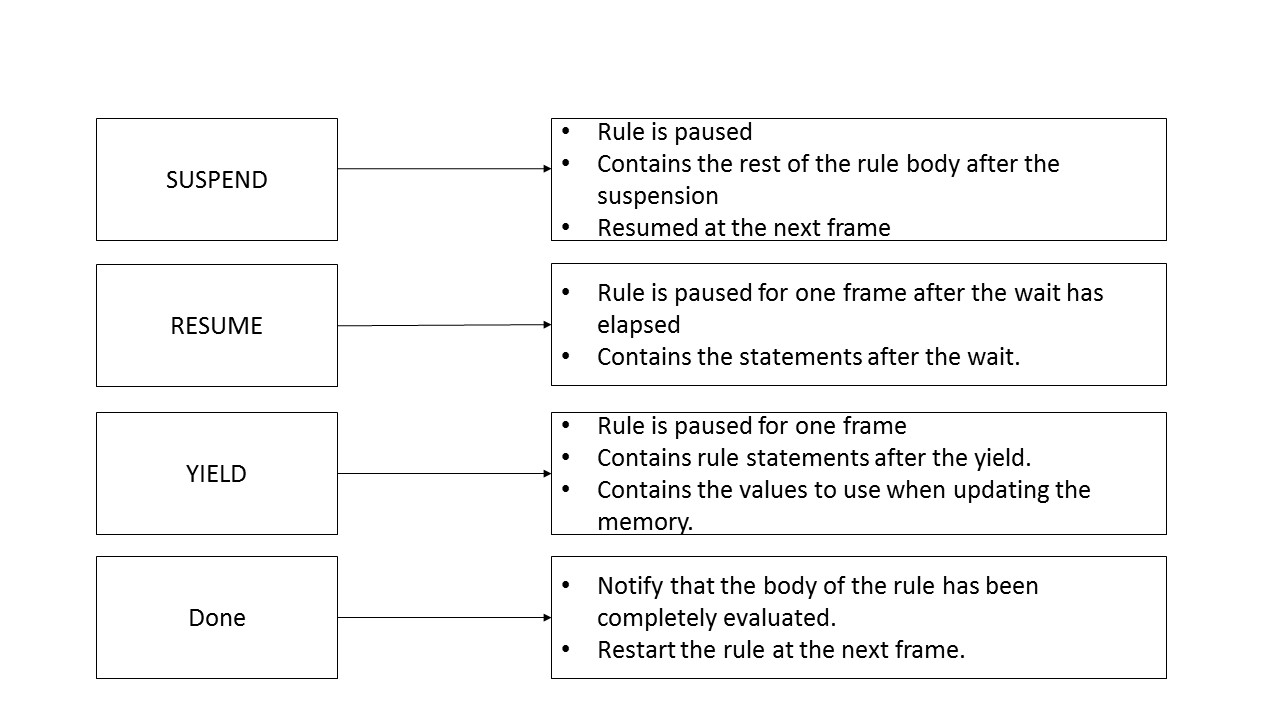
\includegraphics[scale = 0.25]{Figures/tick2}
	\caption{Casanova 2.5 rule evaluation}
	\label{fig:tick}
\end{figure}

The function \texttt{evalRule} calls \texttt{evalStatement} to evaluate the first statement in the body of the rule passed as argument. The result of the evaluation of the statement is processed in the following way: (\textit{i}) if the result is \texttt{Done}, \texttt{Suspend} or \texttt{Resume} then it is just returned to the caller function. We omit the code for this case, since it is trivial; (\textit{ii}) if the result is \texttt{Atomic} it means that the evaluated statement was uninterruptible and the remaining statements of the rule must be re-evaluated immediately; (\textit{iii}) if the result is \texttt{Yield} then the fields in the domain are updated recursively in order and then the updated memory is encapsulated in the \texttt{Yield} data structure and passed to the caller function.

\vspace{0.1cm}
\begin{lstlisting}
evalStatement b k ctxt dt => Atomic z c    
evalRule (rule dom z nop c dt) => res
-------------------------------
evalRule (rule dom b k ctxt dt)  => res
\end{lstlisting}

\begin{lstlisting}
evalStatement b k (Context locals fields globals) dt => Yield ks values context
updateFields dom values context  => updatedContext
--------------------------------------------------------
evalRule (rule dom b k locals dt) fields globals => Yield ks values updatedContex
\end{lstlisting}

Note that, in case of a rule containing only atomic statements, we will eventually return \texttt{Done} after having recursively called \texttt{evalStatement} for all the statements, and the rule will be paused for one frame.

\begin{comment}
\begin{figure}
\centering
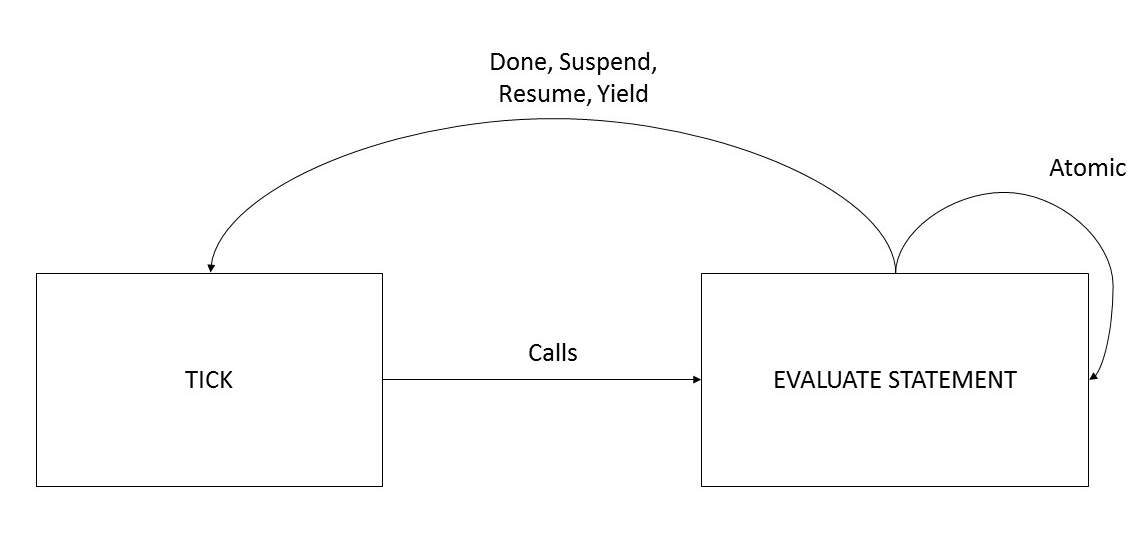
\includegraphics[scale=0.15]{Pictures/statement_evaluation}
\caption{Statement evaluation}
\label{fig:statement_evaluation}
\end{figure}
\end{comment}

\noindent
The \texttt{evalStatement} function is used both to evaluate a single statement and a sequence of statements. When evaluating a sequence of statements, the first one is extracted. A continuation is built with the following statement and passed to a recursive call to \texttt{evalStatement} which evaluates the extracted statement. If the existing continuation is non-empty, then it is added before the current continuation. If both the continuation and the body are empty (situation represented by the \texttt{nop} operator) then it means the rule evaluation has been completed and we return \texttt{Done}.

\begin{lstlisting}
a != nop
---------------------                           ----------------------- 
addStmt a b => a;b                              addStmt nop nop => nop   

addStmt b k => cont
evalStatement a cont ctxt dt => res
-------------------------------                 -----------------------------------       
evalStatement (a;b) k ctxt dt => res            evalStatement nop nop ctxt dt => Done ctxt


\end{lstlisting}

\noindent
We will now present, for brevity, only the evaluation of the \texttt{wait} and \texttt{yield} statements. Both the evaluation of the control structures and the variable bindings always return \texttt{Atomic} because they do not, by definition, pause the execution of the rule.

The \texttt{wait} statement has two different evaluations, based on the rules defined in Section \ref{sec:problem_statement}: (\textit{i}) the timer has elapsed: in this case we return \texttt{Resume} which contains the code to execute after the \texttt{wait} statement, or (\textit{ii}) the timer has not elapsed: in this case we return \texttt{Suspend} which contains the \texttt{wait} statement with the updated timer followed by the continuation.


\begin{lstlisting}
<<t <= dt>> == false
----------------------------------
evalStatement (wait t) k ctxt dt => Suspend wait <<t - dt>>;k ctxt

<<t <= dt>> == true
----------------------------------
evalStatement (wait t) k ctxt dt => Resume k ctxt
\end{lstlisting}

\noindent
The \texttt{yield} statement takes as argument a list of expressions whose values are used to update the corresponding fields in the rule domain. The evaluation rule recursively evaluates the expressions and stores them into a list passed as argument of the \texttt{Yield} result. Those arguments are used later by \texttt{evalRule} to update the corresponding fields.

\begin{lstlisting}
eval expr ctxt => v
evalYield exprs ctxt => vs
-------------------------------------------          ----------------------------
evalYield (expr :: exprs) ctxt => v :: vs            evalYield nil ctxt => nil
\end{lstlisting}

In this section we provide an implementation of a patrol script for an entity in a game. The sample is made up of an entity, representing a guard, and a couple of checkpoints. The guard continuously moves between the two checkpoints. We choose this sample because this is a typical behaviour implemented in several games, where the user is able to set up a patrol route for a unit. We show the comparison between the sample implemented in Casanova 2.5 and an equivalent implementation in Python with respect to the running time. We then show a comparison between the hard-coded compiler of Casanova 2.0 and the implementation of Casanova 2.5 in Metacasanova with respect to the code length. 

\begin{comment}
We want to underline that the main goal of this work is \textbf{to ease the process of building a compiler for a DSL for games, thus our main objective is decreasing the code length and complexity necessary to implement a hard-coded compiler for the language}. At the same time we show that the compiled program in Casanova 2.5 \textbf{has performance similar to that of a language used in game development, and thus Casanova 2.5 is usable in a real scenario}.
\end{comment}

\subsection{Chosen languages}
We compared the running time of the sample in metacompiled Casanova with an equivalent implementation in Python. This language was chosen based on its use in game development: Python has been used extensively in several games such as Civlization IV \cite{CIV4} or World in Conflict \cite{WIC} because of the native support for coroutines. We deliberately ignore C++ and C\# implementations, although they are widely used in the industry, because we knew in advance \cite{CASANOVA2_PAPER} that the current version of the code generated by the meta-compiler would not match the high performance of these languages: the main goal of this work is to reduce the effort of writing a compiler for a DSL for games while having acceptable performance.


\subsection{Performance}
The performance results are shown in Table \ref{tab:evaluation}. We see that the generated code has performance on the same order as Python. This is mainly due to the fact that the memory, in the metacompiled implementation of Casanova, is managed through a map, and because of the virtuality of the implemented operators. Each time Casanova accesses a field in an entity this must be looked up into the map. To this we add the complexity of dynamic lookups when we must deal with polymorphic results into the rules. 

From Table \ref{tab:compiler_comparison} we see that the implementation of Casanova 2.0 language in Metacasanova is almost 5 times shorter in terms of lines of code than the previous Casanova implementation in F\#. We believe it is worthy noticing that structures with complex behaviours, such as \textit{wait} or \textit{when}, require hundreds of lines of codes with a standard approach (the code lines to define the behaviour of the structure plus the support code to correctly generate the state machine), while in the meta-compiler we just need tens of lines of codes to implement the same behaviour. Moreover we want to point out that the previous Casanova compiler was written in a functional programming language: these languages tend to be more synthetic than imperative languages, so the difference with the same compiler implemented in languages such as C/C++ might be even greater.

The readability with respect to the hard-coded compiler code is also improved: we managed to implement the behaviour of synchronization and timing primitives almost imitating one to one the formal semantics of the language definition (see the semantics rules in Section \ref{sec:formal_description} and their implementation in Section \ref{sec:casanova3}). In the hard-coded compiler implementation for Casanova 2.0 the semantics are lost in the code for generating finite state machines.

\begin{table}[!h]
	\centering
	\tiny	
	\begin{tabular}{|c|c|c|}
		\hline
		\multicolumn{3}{|c|}{\textbf{Casanova 2.5}} \\
		\hline
		Entity \# & Average update time (ms) & Frame rate \\
		\hline
		100 & 0.00349 & 286.53 \\
		\hline
		250 & 0.00911 & 109.77 \\
		\hline
		500 & 0.01716 & 58.275 \\
		\hline
		750 & 0.02597 & 38.506 \\
		\hline
		1000 & 0.03527 & 28.353 \\
		\hline
		\multicolumn{3}{|c|}{\textbf{Python}} \\
		\hline
		Entity \# & Average update time (ms) & Frame rate \\
		\hline
		100 & 0.00132 & 756.37 \\
		\hline
		250 & 0.00342 & 292.05 \\
		\hline
		500 & 0.00678 & 147.54 \\
		\hline
		750 & 0.01087 & 91.988 \\
		\hline
		1000 & 0.01408 & 71.002 \\
		\hline
	\end{tabular}
	\caption{Patrol sample evaluation}
	\label{tab:evaluation}
\end{table}

\begin{table}[!h]
	\centering
	\tiny
	\begin{tabular}{|c|c|}
		\hline
		\multicolumn{2}{|c|}{\textbf{Casanova 2.5 with Metacasanova}} \\
		\hline
		Module & Code lines \\
		\hline
		Data structures and function definitions & 40 \\
		\hline
		Query Evaluation & 16 \\
		\hline
		While loop & 4 \\
		\hline
		For loop & 5 \\
		\hline
		If-then-else & 4 \\
		\hline
		When & 4 \\
		\hline
		Wait & 6 \\
		\hline
		Yield & 10 \\
		\hline
		Additional rules for Casanova program evaluation & 40 \\
		\hline
		Additional rules for basic expression evaluation & 201 \\
		\hline
		\multicolumn{2}{|l|}{\textbf{Total: } 300} \\
		\hline
		\multicolumn{2}{|c|}{\textbf{Casanova 2.0 compiler}} \\
		\hline
		Module & Code lines \\
		\hline
		While loop & 10 \\
		\hline
		For-loop and query evaluation & 44 \\
		\hline
		If-Then-Else & 15 \\
		\hline
		When & 11 \\
		\hline
		Wait & 24 \\
		\hline
		Yield & 29 \\
		\hline
		Additional structures for rule evaluation & 63 \\
		\hline
		Structures for state machine generations & 754 \\
		\hline
		Code generation & 530 \\
		\hline
		\multicolumn{2}{|l|}{\textbf{Total: } 1480} \\
		\hline			
	\end{tabular}	
	\caption{meta-compiler vs standard compiler}
	\label{tab:compiler_comparison}
\end{table}

\subsection{Discussion}
\label{subsec:code_generation_discussion}
Metacasanova has been evaluated in \cite{DiGiacomo2017} by re-building the DSL for game development Casanova \cite{abbadi2015casanova, abbadithesis2017}. Even though the size of the code required to implement the language has been drastically reduced (almost 1/5 shorter), performance dropped dramatically. We identified a main problem causing the performance decay that, if solved, will improve the performance of the generated code.

In order to encode a symbol table in the meta-compiler in the current implementation (used for example to store the variables defined in the local scope of a control structure or to model a class/record data structure), we are left with two options: (\textit{i}) define a custom data structure made of a list of pairs, containing the field/variable name as a string and its value, in the following way

\begin{lstlisting}
Data "table" -> List[Tuple[string, Value]] : SymbolTable
\end{lstlisting}

\noindent
or (\textit{ii}) use a dictionary data structure coming from .NET, such as \texttt{ImmutableDictionary}, which was the implementation choice for Casanova. In both cases, the behaviour of the language implemented in Metacasanova will be that of a dynamic language, because whenever the value of a variable or class field must be read, the evaluation rule must look up the symbol table at run time to retrieve the value, whose complexity will be $O(n)$ with the list implementation and $O(\log n)$ with the dictionary implementation. This issue is caused by the fact that, in the current state of Metacasanova, the meta-type system is unaware of the type system of the language that is being implemented in the meta-compiler. This is not a problem limited to Metacasanova but to all meta-compilers having a meta-type system that does not allow embedding of the host language type system. In the next section we propose an extension to Metacasanova to overcome this problem by embedding the type system of the implemented language in the meta-type system of Metacasanova and inlining the code to access the appropriate variable at compile time.